\label{Ch:4}
In this section, we describe our data-driven inverse reinforcement learning based social navigation pipeline.\\
%\\ \textbf{An image showing the block diagram of the pipeline including the environment, the feature extractor, and the other components}

\begin{figure}[!htbp]
	\centering
	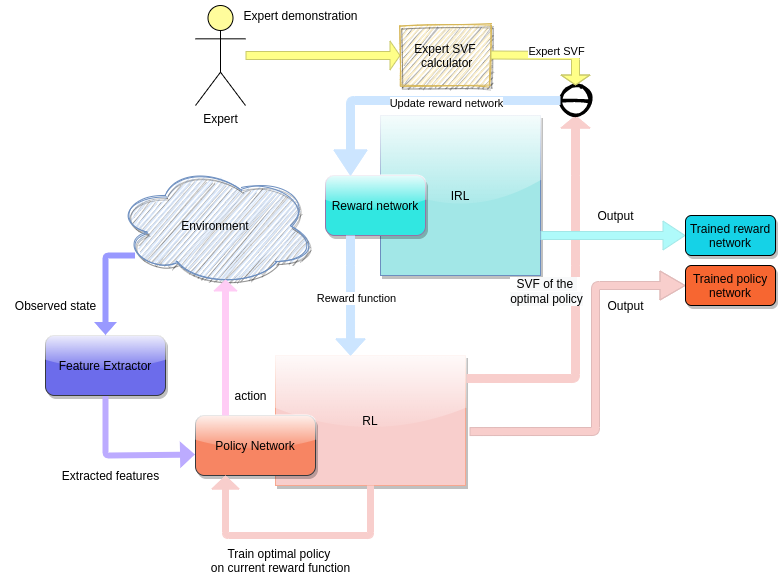
\includegraphics[width=\linewidth]{figures/irl_pipeline.png}
	\caption{An overview of the proposed navigation pipeline.}
	\label{fig:irl_pipeline}
\end{figure}

\section{The IRL block:}
Inverse reinforcement learning(IRL) or inverse optimal control (IOC) has been greatly explored to train robots in real-world tasks.The appeal of IRL is that there is no need to specify a reward function that dictates the optimal behavior of an agent. Instead, the optimal or desired behavior can be obtained from a set of expert demonstrations which is more readily available compared to an artificially constructed reward structure as needed in reinforcement learning (RL).

To keep the chapter self-contained, we will recap our definition of a Markov decision process (MDP):
A Markov decision process or MDP can be defined as a tuple ($\mathcal{S}$,$\mathcal{A}$,T,$\gamma$, $\mathcal{R}$)  where,
\begin{itemize}
    \item $\mathcal{S}$ is the set of all possible states.
    \item $\mathcal{A}$ is the set of all possible actions.
    \item T is the state transition dynamics, i.e. the probability of moving to a state given its previous state and action, $P(s^{'}|s, a)$.
    \item $\gamma$ is the discounting factor.
    \item $\mathcal{R}$ is the set of rewards $R:  \mathcal{S} \mapsto \mathbb{R} $ is the reward function. In practice, instead of using the raw states, hand-engineered features are extracted from the states which are then used to calculate the reward of a particular state. This alleviates a lot of complexity when dealing with large continuous state-spaces. 
    \end{itemize}  
The goal of IRL is to infer a reward function that best explains the behavior of the expert. The expert behavior is represented in terms of expert demonstrations or trajectories, $\mathbf{D} = \{ \tau_1, \tau_2, \tau_3, \dots, 
\tau_{M} \}$ in the context of navigation. Each of these trajectories, in turn, can be further broken down into a collection of states $\tau_{i} = \{ s_{0}, s_{1}, s_{2}, \dots, s_{T} \}$ as visited by the expert in the trajectory. \\
\cite{abbeel_apprenticeshiplearning_2004} shows that solving the Bellman equations for an analytic solution to obtain the reward $\mathcal{R}$ is under-constrained. \cite{ziebart_maxent_2008} addresses this by introducing an entropy-based constraint \cite{jaynes1957information} on the distribution of the trajectories which state that the probability of the occurrence of a trajectory is directly proportional to the reward it receives which is equal to the summation over the reward it receives at each state in the trajectory.
\begin{align}
P(\tau_{i}| \theta) = \frac{1}{Z(\theta)}\exp^{\theta^{T}\mathbf{f}_{\tau_{i}}} = \frac{1}{Z(\theta)}\exp^{\sum_{s_{j}\in\tau_{i}}\theta^{T}\mathbf{f}_{s_{j}}}
\end{align}
\begin{align}
Z = \sum_{\tau_{i}\in \mathbf{D}}\exp{\theta^{T}\mathbf{f}_{\tau_{i}}}
\end{align}
where, $Z$ is the normalizing term, and $\mathbf{D}$ is the set of all possible trajectories.\\
Given a set of expert demonstrations, an optimal reward structure should maximize the probability of the occurrence of the expert demonstrations and their associated states. Mathematically, this is given by: 
\begin{align}
\label{eq:loglikelihood-IRL}
\theta^{*} = \argmax_{\theta} \mathbf{L}(\theta) = \argmax_{\theta} \sum_{\tau \in D} \log{P(\tau| \theta, T)}
\end{align}
\cite{ziebart_maxent_2008} uses a linear combination of weights as the reward function which is limiting in expressing complex reward functions. This problem is addressed by Wulfmeier et al. where they restructure the maximum entropy IRL formulation using neural networks \cite{wulfmeier2015maximum}. Neural networks are universal function approximators. This vastly increases the amount of complexity a reward function can express.\\
The parameters of a neural network represented by $\theta$ can be found using gradient descent methods. The  update term for the reward network parameters w.r.t. the loss term $\mathbf{L}$ is equal to the difference in the state visitation frequencies (SVF) of the expert demonstrations and the policy $\pi_{\psi} : \mathcal{S} \mapsto \mathcal{A} $ trained on the parameters of the current reward network $R_{\theta}$:
\begin{align}
	\label{eq:IRL-parameter-update-states}
	\frac{\partial L}{\partial \theta} = \left(\sum_{\tau_{i} \in D}\sum_{s_{j} \in \tau{i}}s_{j} - \sum_{\hat{\tau} \in \hat{D}}\sum_{s_{k} \in \hat{\tau}}s_{k}\right)
\end{align}
where, $\hat{\tau}$ is a trajectory sampled by the policy $\pi_{\psi}$.\\
Replacing a state, $s_{i}$, by its features, $\phi(s_{i})$, \autoref{eq:IRL-parameter-update-states} can be re-written as:
\begin{align}
	\label{eq:IRL-parameter-update-features}
	\frac{\partial L}{\partial \theta} = \left(\expectval_{s \sim P(s|\mathcal{D})} \phi(s) - \expectval_{s \sim P(s|\pi_\psi)} \phi(s)\right) \frac{\partial R_\theta}{\partial \theta} 
\end{align}
\subsection{The SVF calculation}
One of the main challenges of IRL is calculating the expected state distribution or the state visitation frequency (SVF) of a policy $\phi_{\psi}$. In model-based environments, this can be calculated using the state transition matrix and dynamic programming \cite{wulfmeier2015maximum}. Access to the actual state dynamics of an environment, especially in real-world applications like navigation, is difficult and not readily available. Instead, we relax this assumption for a model-free but deterministic environment. This is a reasonable assumption in the context of a navigation problem because the movements of pedestrians, in general, are inherently deterministic. %and any observed uncertainty by the agent can be attributed to the error in measurement by the onboard sensors.\\

We use sampling to get an estimate of the SVF. While this can be time-consuming and computationally expensive, the task is drastically simplified when using greedy policies, especially in a deterministic environment. SVF calculation of a greedy policy in a deterministic environment can be calculated by taking a single sample trajectory (due to the deterministic nature of the environment) for each pedestrian by replacing them with the agent and letting it run till completion. The calculation of the expected state visitation frequency of the agent is shown in equation \autoref{eq:svf-sampling}

\begin{align}
\label{eq:svf-sampling}
   \expectval_{s \sim P(s|\pi_\psi)} \phi(s) \approx \sum_{s_0 \in p_0} \sum_{t=0}^{T} \phi(\hat{P}(s_{t+1}|s_t, a_t)\pi_\psi(a_t|s_t))
\end{align}
where, $\hat{P}(s_{t+1}| s_{t}, a_{t})$ are the state transitions observed during the process of sampling the trajectories from the environment, and not from a known state transition model.
%The original formulation of maximum entropy deep inverse reinforcement learning (MEDIRL) is in a model-based setting and the state transition matrix is used to calculate the state visitation frequency (SVF) of the agent. While this produces an exact value of the agent's SVF, assuming the availability of the state transition matrix is fairly optimistic for most real-world tasks including navigation. In an attempt to make things less constrained we take the model-free approach and focus on calculating the SVF using a sampling-based method. 
%The SVF calculation:
%The main challenge of going model-free is the calculation of the normalizing factor(Z), which in the presence of a state transition matrix could be calculated using dynamic programming [citation of the paper]. 
%Under the assumption of a model-free but deterministic environment, the SVF of a policy can be reasonably computed by taking trajectory samples from the starting context of each of the existing pedestrians in the scene once. 
%\begin{align}
%equation 4 from iros2020
%\end{align}
%where the $\mathcal{P}$ represents state transitions obtained from sampling and not the state transition dynamics. \textbf{We argue that this assumption is reasonable in a navigation setting because the task is not inherently uncertain, and most transition dynamic uncertainty can be attributed to sensory noise and control error. We summarize our approach in algorithm 1. (Taken word-to-word from IROS manuscript)}
\begin{algorithm}[tbhp]
	\caption{Deterministic Maximum Entropy IRL}
	\label{deterministic-medirl}
	
	\SetKwInOut{Input}{Input}
	\SetKwInOut{Output}{Output}
	
	\Input{$D, \gamma, p_0$}
	
	\SetKwComment{Comment}{$\triangleright$\ }{}
	\SetKwFunction{Backprop}{Backprop}
	\SetKwFunction{UpdateWeight}{UpdateWeight}
	\SetKwFunction{SolveMDP}{SolveMDP}
	\BlankLine
	$\theta, \psi \gets \theta_0, \psi_0$ \DontPrintSemicolon \Comment*[r]{Initialize parameters} 
	$\mu_e= \expectval_{s \sim D}{\phi(s)}$ \DontPrintSemicolon \Comment*[r]{Calculate expert svf}
	\For{$m \gets 1$ \KwTo M}{
		$\pi_\psi^m \gets \SolveMDP(R_\theta^m,\mathcal{S}, \mathcal{A}, \mathcal{T}, \gamma)$\\
		$\mu_{\text{svf}} = \mu_e - \expectval_{s \sim P(s|\pi_\psi^m)} \phi(s)$ \Comment*[r]{from \autoref{eq:svf-sampling}} 
		$\frac{\partial L}{\partial \theta^m} = $ \Backprop($\theta^m, \mu_{\text{svf}}$) \\
		$\theta^{m+1} \gets $ \UpdateWeight($\frac{\partial L}{\partial \theta^m}, \theta^m$) 
	}
	\BlankLine
	\Output{optimal parameters $\theta, \psi$}
	
\end{algorithm}

The expert policy needs to be retrained every time the parameters of the reward network are updated. We solve the MDP using an actor-critic method \cite{mnih_actor_critic_2016}.

%\subsection*{Overview of the algorithm used}
%The algorithm trains for two networks, the reward network that, given the features of a state returns the reward associated with it,\\
%\textbf{equation}\\ stating this.
%and the policy network, which given the same, returns the best possible action.\\
%\textbf{equation}\\
%The method starts with randomly initializing the weights of the reward network. This reward network is then used in the  RL block to train an agent which is optimal for the current reward structure. Once, an optimal policy is obtained, the policy is then sampled from, in the environment to obtain roll-outs or trajectories in this case. A trajectory is given by the sequence of states visited by the agent {s1, s2, ... sn}.
%Once the trajectories are obtained, they are used to calculate the state visitation frequency. The difference between the expert and the agent SVF is used to calculate the loss
%\textbf{equation}
%This loss is then backpropagated through the reward network to update the weights.
%Once the weights are updated, the new network is again fed into the RL block. This iterative process continues until completion.
%Explanation of the L1 regularization over l2 regularization 

\section*{The RL block:}

Actor-critic are a class of reinforcement learning algorithms that are built upon policy gradient methods. 
In policy-gradient methods, the goal is to iteratively improve the performance of a given policy. This is achieved by maximizing the expected return of the policy. Mathematically, the objective of a policy gradient method can be expressed as:
\begin{align}
maximize \;\; J( \psi )  &\; = \; \mathbb{E} [ R | \pi_{\psi} ] \\
                       & \; = \; \mathbb{E}[ \sum^{T-1}_{t=0} r_{t+1}| \pi_{\psi}] 
\end{align}
where, $r_{t}$ is the reward obtained at time $t$ and $\pi_{\psi}$ is the policy with parameters $\psi$.\\
This leads to an update function:
\begin{align}
\label{eq:policy-gradient-update}
\nabla_{\psi} J (\psi) = \sum_{t=0}^{T-1} \nabla_{\theta}\log \pi_{\psi}(a_{t}|s_{t})\sum_{t'=t+1}^{T} \gamma^{t'-t-1} r_{t'}
\end{align} 
where, $\sum_{t'=t+1}^{T} \gamma^{t'-t-1} r_{t'}$ is the cumulative discounted reward obtained by following the policy $\pi_{\psi}$ from time $t'$.\\
Vanilla policy gradient methods suffer from high variance because they do not have a normalizing factor for the second term. This is addressed by introducing a baseline. The baseline can be calculated in various ways. One of the resulting algorithms is the A2C or the Advantage actor-critic algorithm \cite{mnih_actor_critic_2016}, where the 'advantage' is the difference between the estimated value of a state at time $t$, $V(s_t)$ and the discounted cumulative reward obtained by following the policy: $\sum_{t'=t+1}^{T} \gamma^{t'-t-1} r_{t'}$. \\
Instead of having two separate networks for the actor(policy) and the critic(value), we design the network in a way that the actor, $\psi_{a}$, and the critic, $\psi_{c}$, share parameters in input and the hidden layers, with a dedicated output layer for the action and value respectively.
\begin{align}
\label{eq:advantage-actor-update}
\nabla_{\psi} J (\psi_{a}) = & \sum_{t=0}^{T-1} \nabla_{\theta}\log \pi_{\psi}(a_{t}|s_{t}) \left(\sum_{t'=t+1}^{T} \gamma^{t'-t-1} r_{t'} - V_{v}(s_{t})\right)\\
\label{eq:advantage-critic-update}
\nabla_{\psi} J (\psi_{c}) = & \sum_{t=0}^{T-1} \left(\sum_{t'=t+1}^{T} \gamma^{t'-t-1} r_{t'} - V_{v}(s_{t})\right)
\end{align} 
where \autoref{eq:advantage-actor-update} is the update for the parameters of the actor network $\psi_{a}$, and \autoref{eq:advantage-critic-update} is for the critic network $\psi_{c}$. 
%The A2C method:
%Two symbiotic agents at play here. The actor and the critic. 
%The critic estimates the value function of a given state.
%The actor uses this information to update its policy distribution.
\vfill
\begin{algorithm}[tbhp]
	\caption{RL algorithm: Actor Critic}
	\label{alg:actor-critic}
	\SetKwInOut{Input}{Input}
	\SetKwInOut{Output}{Output}
	\Input{$R, \gamma, p_0$}
	
	\SetKwComment{Comment}{$\triangleright$\ }{}
	\SetKwFunction{Backprop}{Backprop}
	\SetKwFunction{UpdateWeight}{UpdateWeight}
	\SetKwFunction{SolveMDP}{SolveMDP}
	\BlankLine
	$\psi \gets \psi_0$ \DontPrintSemicolon \Comment*[r]{Initialize parameters} 

	\For{$m \gets 1$ \KwTo M}{
		Sample $\{s_{i}, a_{i} \}$ from $\pi_{\psi}$ till termination of an episode.\\
		$\hat{A}(s_{i}, a_{i})$ = $\sum_{t'=i+1}^{T} \gamma^{t'-i-1} r_{t'} - \pi_{\psi_{c}}(s_{i})$ \Comment*[r]{Calculate advantage}
		$\mathbf{L_{act}}$ = $\sum \log{\pi_{\psi_{a}}(a_{i}| s_{i})}\hat{A}(s_{i}, a_{i})$  \Comment*[r] {Calculate actor loss}
$\mathbf{L_{crit}}$ = $\sum \hat{A}(s_{i}, a_{i})$ \Comment*[r]{Calculate critic loss}
		$\frac{\partial \mathbf{L}}{\partial \psi^m} \gets $ \Backprop($\mathbf{L}_{act} + \mathbf{L}_{crit}$) \\
		$\psi^{m+1} \gets $ \UpdateWeight($\frac{\partial \mathbf{L}}{\partial \psi^m}, \psi^m$) 
	}	
	\BlankLine
	\Output{optimal parameters $\psi$}
	
\end{algorithm}


\section{The Feature extractor}
The feature extractor is a vital component in the navigation pipeline. It is the medium that facilitates interaction between the learning algorithm and the environment and heavily influences the performance of the agent \cite{vasquez_inverse_2014}. We assume the following information available to us: the current position and velocity of the agent, the position of the goal, and the position and velocity of all the pedestrians present in the frame. Although we have access to information about all the pedestrians, the feature representations are designed to be calculated from a partial observation of the environment.\\
The feature representation consists of the following components:
\begin{itemize}
    \item The \textbf{local component} contains information from the vicinity of the agent captured in the form of a binary feature vector. This provides an approximate idea of the nearby obstacles and an estimate of a likely collision. Hence the term: 'risk-features'. 
    \item The \textbf{global component}, on the other hand, provides an approximation of the goal location on the map. 
\end{itemize}
 We assume the following information available to us: the current position and velocity of the agent, the position of the goal, and the position and velocity of all the obstacles (pedestrians) in the current frame.  Having access to all this information using sensors on a mobile robot navigating the real world is highly unlikely and difficult to obtain. This is additionally addressed by the feature extractor, which also acts as an information moderator, receiving raw information from the environment and packaging it in a feature vector that can be readily constructed by a mobile robot on the go using off-the-shelf sensors.\\
 Both the local and the global components along with their sub-components are described in greater detail below.
Talk about the relative orientation calculation


\subsection*{The global component}
The global information is further comprised of 3 elements:

\subsubsection*{Relative goal orientation} 
This acts as a compass, providing a rough estimate of the direction of the goal based on the current position and orientation of the agent. This is denoted by a $9 \times 1$ one-hot vector, where the presence of the goal in any one of the bins is marked by a $1$ keeping the rest to $0$. The $360 \degree$ around the agent is divided into $8$ equal divisions forming the first 8 bins of $45 \degree$ each. The $9^{th}$ bin denotes the contact of the agent with the goal.
\begin{table}[tbhp]
	\label{tab:goal-vector-bins}
	\begin{center}
		\begin{tabular}{|c|c|}
			\hline
			Feature & Threshold \\
			\hline
			$\phi_{GV1}$ & $\alpha_{GV} \in \left[ \frac{15\pi}{8} , 2\pi \right) \cup \left[ 0, 2\pi \right)$ \\
			
			$\phi_{GV2}$ & $\alpha_{GV} \in \left[ \frac{\pi}{8} , \frac{3\pi}{8} \right)$ \\
			
			$\phi_{GV3}$ & $\alpha_{GV} \in \left[ \frac{3\pi}{8} , \frac{5\pi}{8} \right)$ \\
			
			$\phi_{GV4}$ & $\alpha_{GV} \in \left[ \frac{5\pi}{8} , \frac{7\pi}{8} \right)$ \\
			
			$\phi_{GV5}$ & $\alpha_{GV} \in \left[ \frac{7\pi}{8} , \frac{9\pi}{8} \right)$ \\
			
			$\phi_{GV6}$ & $\alpha_{GV} \in \left[ \frac{9\pi}{8} , \frac{11\pi}{8} \right)$ \\
			
			$\phi_{GV7}$ & $\alpha_{GV} \in \left[ \frac{11\pi}{8} , \frac{13\pi}{8} \right)$ \\
			
			$\phi_{GV8}$ & $\alpha_{GV} \in \left[ \frac{13\pi}{8} , \frac{15\pi}{8} \right)$ \\
			\hline
		\end{tabular}
	\end{center}
	\caption{Bin thresholds for goal vector features.}
\end{table}

\begin{figure}[tbhp]
	\centering
	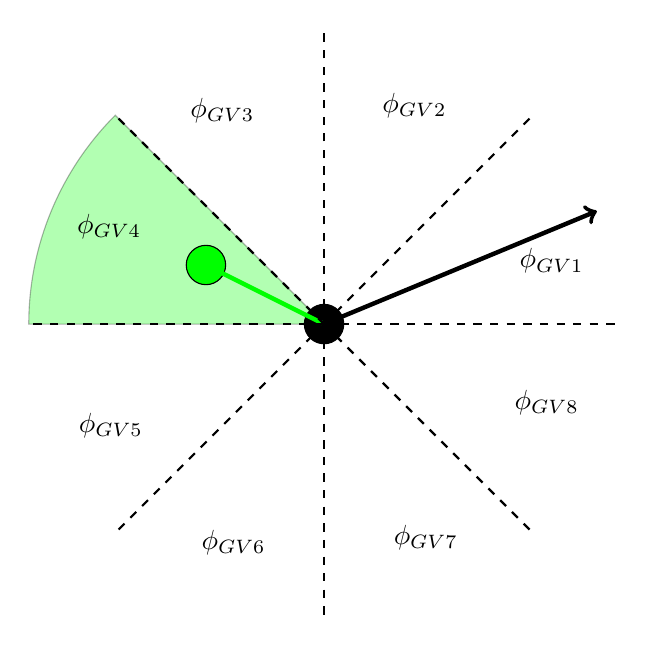
\begin{tikzpicture}[scale=2.5]
	
	\fill [fill=green, opacity=0.0] (0.0,0.0) circle [radius=1.5];
	\draw [fill=green, opacity=0.3] 
	(0,0) -- (-1.5,0) arc(180:135:1.5) -- cycle;
	
	\draw [fill=black] (0,0) circle [radius=0.1];
	\draw [->, ultra thick] (0,0) -- (22.5:1.5);
	
	\draw [fill=green] (-0.6,0.3) circle [radius=0.1];
	\draw [->, ultra thick, green] (0,0) -- (-0.6,0.3);
	
	\draw [dashed, thick] (0,0) -- (0:1.5);
	\draw [dashed, thick] (0,0) -- (45:1.5);
	\draw [dashed, thick] (0,0) -- (90:1.5);
	\draw [dashed, thick] (0,0) -- (135:1.5);
	\draw [dashed, thick] (0,0) -- (180:1.5);
	\draw [dashed, thick] (0,0) -- (225:1.5);
	\draw [dashed, thick] (0,0) -- (270:1.5);
	\draw [dashed, thick] (0,0) -- (315:1.5);
	
	
	
	
	\node at (15.5:1.2) {$\phi_{GV1}$};
	\node at (67.5:1.2) {$\phi_{GV2}$};
	\node at (115.5:1.2) {$\phi_{GV3}$};
	\node at (155.5:1.2) {$\phi_{GV4}$};
	\node at (205.5:1.2) {$\phi_{GV5}$};
	\node at (247.5:1.2) {$\phi_{GV6}$};
	\node at (295.5:1.2) {$\phi_{GV7}$};
	\node at (340.5:1.2) {$\phi_{GV8}$};
	
	\end{tikzpicture}
	
	\caption{Goal vector bin representation. The black disk at the center of the diagram and the black arrow represents the agent's position and heading respectively. The green disk depicts the goal position, and since it lies in $\phi_{GV4}$ that bin is currently active. Note that the features are relative to the agent's orientation and are thus turning with the agent.}
	\label{fig:goal-vector-diagram}
\end{figure}

\subsubsection*{Change in orientation}
Represented by a $5 \times 1$ one-hot vector, the change in orientation captures the magnitude of the change in the orientation of the agent in consecutive steps. The value ranges between $0 \degree$ -  $ 180 \degree$. This value is binned in one of 5 asymmetric bins. The rationale behind the uneven distribution is that empirically we have observed that human motion is smooth. So, the bins are constructed in a way to put greater emphasis on smaller changes in orientation. This helps capture the nuances in human motion in greater detail leading to better encapsulation of the essence of the navigational pattern. The division of the range is shown below.

\begin{table}[htbp]
    \caption{Bin thresholds orientation change features.}
    \label{orientation-change-bins}
    \begin{center}
        \renewcommand{\arraystretch}{1.3}
        \begin{tabular}{|c|c|}
            \hline
            Feature & Threshold \\
            \hline
            $\phi_{O1}$ & $\alpha_{OC} \in \left[ 0 , \frac{\pi}{9} \right)$ \\
            
            $\phi_{O2}$ & $\alpha_{OC} \in \left[ \frac{\pi}{9} , \frac{2\pi}{9} \right)$ \\
            
            $\phi_{O3}$ & $\alpha_{OC} \in \left[ \frac{2\pi}{9} , \frac{3\pi}{9} \right)$ \\
    
            
            $\phi_{O5}$ & $\alpha_{OC} \in \left[ \frac{3\pi}{9} , \frac{4\pi}{9} \right)$ \\
            
            $\phi_{O6}$ & $\alpha_{OC} \in \left[ \frac{4\pi}{9} , \pi \right)$ \\
            \hline
        \end{tabular}
    \end{center}
\end{table}
\subsubsection*{Deviation from the goal}
The deviation from goal captures the magnitude of the angle between the vector to the goal from the current position of the agent and the current orientation vector of the agent. The value ranges from $0 \degree$ - $ 180 \degree$ which is again asymmetrically divided into 4 bins ($4 \times 1$ one-hot vector), with greater emphasis is laid on the lower degrees due to reasons mentioned earlier. 

\begin{table}[htbp]
    \label{deviation-from-goal-bins}
    \begin{center}
        \renewcommand{\arraystretch}{1.3}
        \begin{tabular}{|c|c|}
            \hline
            Feature & Threshold \\
            \hline
            $\phi_{GA1}$ & $\alpha_{GA} \in \left[ 0 , \frac{\pi}{8} \right)$ \\
            
            $\phi_{GA2}$ & $\alpha_{GA} \in \left[ \frac{\pi}{8} , \frac{\pi}{4} \right)$ \\
            
            $\phi_{GA3}$ & $\alpha_{GA} \in \left[ \frac{\pi}{4} , \frac{3\pi}{4} \right)$ \\
            
            $\phi_{GA4}$ & $\alpha_{GA} \in \left[ \frac{3\pi}{4} , \pi \right]$ \\
            \hline
        \end{tabular}
        \caption{Bin thresholds for deviation from the goal.}
    \end{center}
\end{table}

\subsubsection*{Speed}
The current speed of the agent is quantized and represented in the form of a $6 \times 1$ one-hot vector. 

%\begin{table}[htbp]
%    \caption{Thresholds for the qantization of the speed of the agent.}
%    \label{tab:speed-quantization}
%    \begin{center}
%        \renewcommand{\arraystretch}{1.3}
%        \begin{tabular}{|c|c|}
%            \hline
%            Raw speed & Speed bin \\
%            \hline
%            0 - 0.2 & 0 \\
%            0.2 - 0.4 & 1 \\
%            0.4 - 0.6 & 2 \\
%            \hline
%        \end{tabular}
%    \end{center}
%    \end{table}

\subsection*{The local information}
Taking inspiration from previous works in this field \cite{fahad_learning_2018} \cite{vasquez_inverse_2014}, we use spatial bins to effectively divide the region surrounding the agent into discrete segments and calculate a 'risk' metric for each of these bins.

\subsubsection*{Creation of the bins}
There are 16 spatial bins surrounding the agent arranged in two concentric circles. 8 equal divisions of the region between the agent and the inner circle form bin 1-8. Similarly, the divisions in the region between the first and the second concentric circle form bins 9 - 16.
\subsubsection*{Calculation of the risk}
Oxford learner's dictionary defines 'risk' as "a person or thing that is likely to cause problems or danger at some time in the future" \textcolor{red}{cite oxford learners' dictionary}. In this context, 'risk' can be loosely correlated to the likelihood of a collision with a nearby obstacle/pedestrian. As a property of the spatial bins, it implies the possibility of a collision with an obstacle located in the given bin. 
The 'risk' is divided into 3 levels: high, low, and medium.
\begin{itemize}
    \item High risk:
When the relative motion of an obstacle is towards the agent and can lead to a collision if not intervened.
    \item Low risk:
When the relative motion of an obstacle is away from the agent.
    \item Med risk:
Anything in between.
\end{itemize}
The calculation of the risk values are based on the following entities:
\begin{align}
    \vec{o}_{rel} = & \;\; \vec{o}_{obs} - \vec{o}_{agent}  \\
    \vec{d}_{rel} =  &\;\; \vec{d}_{agent} - \vec{d}_{obs} \\
    \theta_{risk} =  & \;\; \angle (\vec{o}_{rel}, \vec{o}_{rel}) \\
    \mathbf{s}_{obs} = & \;\; \tan(\theta_{risk}) \times |\vec{d_{rel}}| \\
    \mathbf{T} = & \;\; \text{agent witdh} + \text{obstacle witdh}
\end{align}
where $\vec{o}_{rel}$ is the relative orientation of the obstacle w.r.t the agent, $\vec{d}_{rel}$ is the relative position of the agent w.r.t to the obstacle, $\theta_{risk}$ is the angle between the vectors, $\vec{o}_{rel}$ and $\vec{d}_{rel}$,  $\mathbf{s}_{obs}$ is the estimated safety margin between the agent and the obstacle and $\mathbf{T}$ is a predefined value which if maintained between the agent and an obstacle should guarantee a collision-free trajectory.\\
An obstacle is marked as 'high risk' when $\theta$ is less than $90\degree$ and the safety margin is less than $\mathbf{T}$. If $\theta$ < $90 \degree$, this indicates that the obstacle is moving away from the agent and hence chances of collision are less and hence low risk. Anything that does not fall in the above two categories are considered as medium risk. The risk calculation conditions and values are summarized in Table \ref{risk-categorization-table}

\begin{table}[htbp]
    \caption{Categorization of the risk.}
    \label{risk-categorization-table}
    \begin{center}
        \renewcommand{\arraystretch}{1.3}
        \begin{tabular}{|c|c|}
            \hline
            Risk value & Risk condition \\
            \hline
            High & $\theta < 90\degree$ \&  $\mathbf{s}_{obs}$ < $\mathbf{T}$   \\
            
            Low & $\theta > 90\degree$\\
            
            Medium & otherwise \\
            \hline
        \end{tabular}
    \end{center}
\end{table}
The risk value of each bin is represented using a $3 \times 1$ one-hot vector. The risk is calculated for individual obstacles present in a bin separately. In the event of a spatial bin containing more than one obstacle with varying degrees of risk, the risk value assigned to that bin is the highest obtained among all the obstacles that fall under that spatial bin.
\begin{figure}[!htbp]
	\centering
	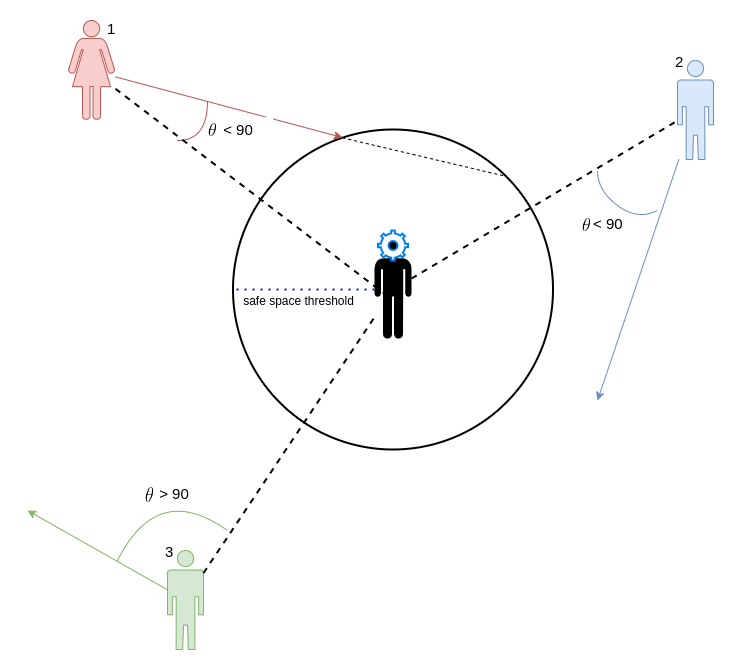
\includegraphics[width=.8\linewidth]{figures/risk_picture.png}
    \label{fig:risk-calculation}
    \caption{A pictorial representation of how the risk is classified. Pedestrian $1$, $2$ and $3$ falls under the category of 'high risk', 'medium' and 'low' risk respectively.}
\end{figure}


%\begin{figure}
%	\label{fig:agent-perspective-risk-features}
%	\begin{subfigure}[t]{.5\linewidth}
%
%		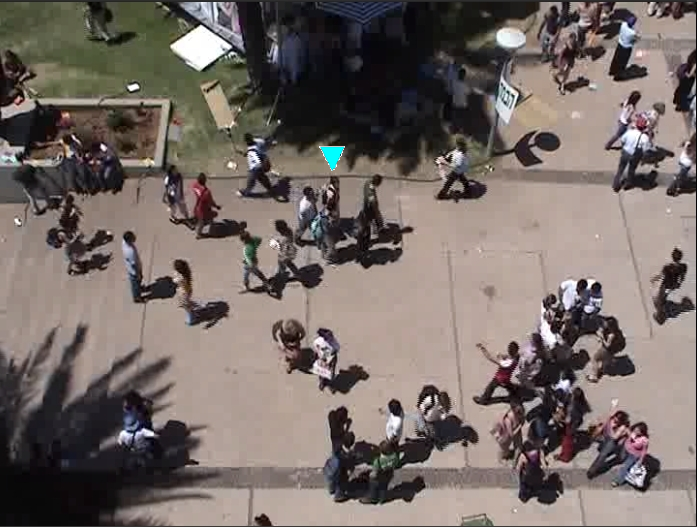
\includegraphics[width=.95\textwidth]{figures/screenshot_video_frame_agent_perspective.png}
%		\label{fig:agent-perspective_screenshot}
%		\caption{A frame from the UCY dataset. The pedestrian which is the acting agent for the current episode is marked with a blue triangle.}
%	\end{subfigure}
%	\begin{subfigure}[t]{.5\linewidth}
%		\centering
%		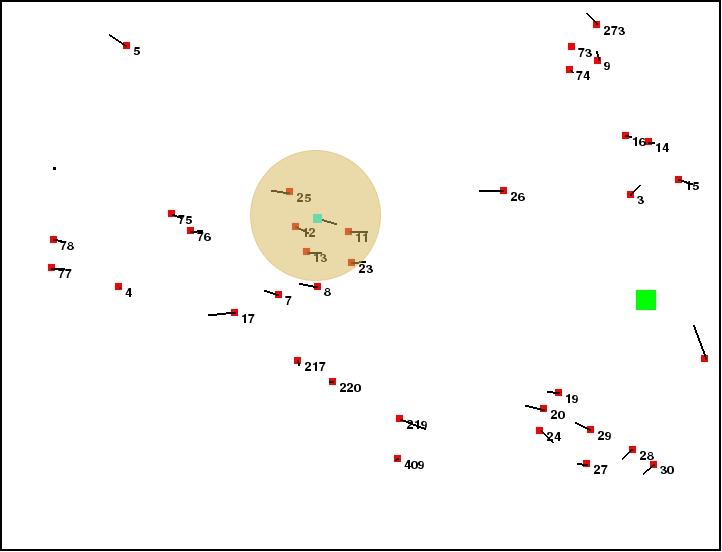
\includegraphics[width=.95\textwidth]{figures/env_screenshot_agent_perspective.png}
%		\label{fig:agent-perspective_env}
%		\centering
%		\caption{Representation of the video frame in the in-house built environment. The blue square represents the acting agent, the red squares represent other pedestrians (obstacles), and the green square represents the goal. The yellow circle around the agent is the area around the agent taken into consideration while computing the local information used by the agent.} 
%	\end{subfigure}
%	\begin{subfigure}[b]{\linewidth}
%		\centering
%		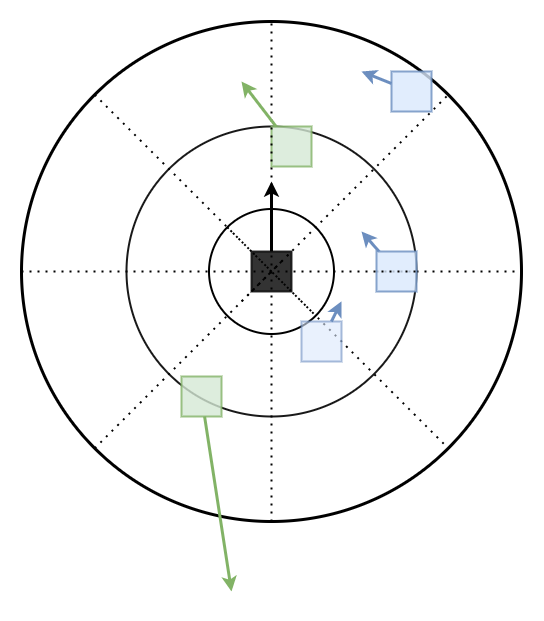
\includegraphics[width=.4\textwidth]{figures/agent_perspective_recreated.png}
%		\label{fig:agent-perspective_agent-perspective}
%		\caption{The local information from the frame as perceived by the agent using the risk features. The spatial bins are represented by the concentric circles around the agent (black square) and the dotted lines. The squares in green mark pedestrians which pose low risk, while the ones in blue denote medium risk.}
%	\end{subfigure}
%\end{figure}


\begin{figure}
	\label{fig:agent-perspective-risk-features}
	\begin{subfigure}[t]{.5\linewidth}
		\centering
		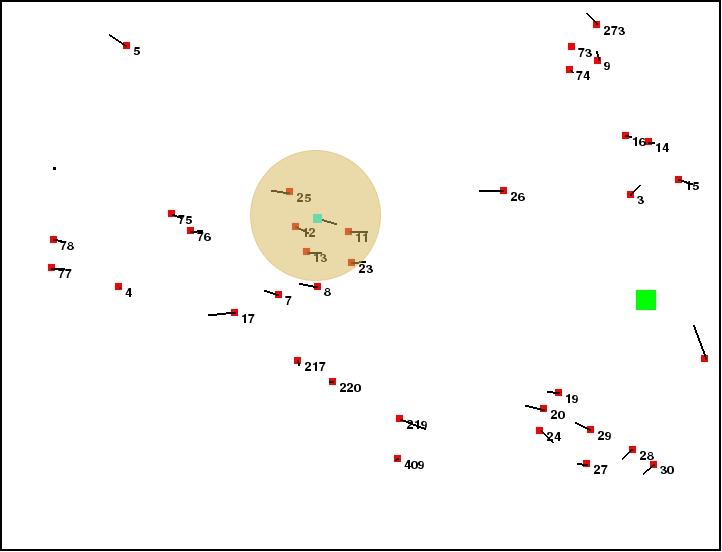
\includegraphics[width=.95\textwidth]{figures/env_screenshot_agent_perspective.png}
		\label{fig:agent-perspective_env}
		\centering
		\subcaption{A screenshot of a frame populated with obstacles.} 
	\end{subfigure}
	\begin{subfigure}[t]{.5\linewidth}
		\centering
		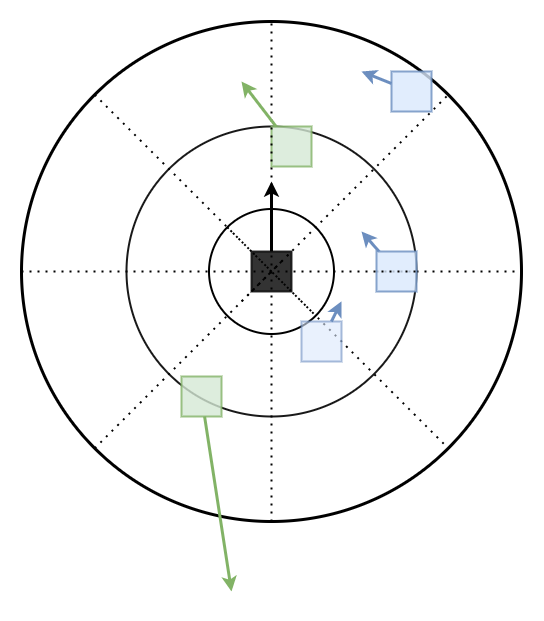
\includegraphics[width=.7\textwidth]{figures/agent_perspective_recreated.png}
		\label{fig:agent-perspective_agent-perspective}
		\subcaption{The local perspective of the agent in the frame. The arrows mark the relative velocity of the nearby pedestrians w.r.t. the agent. Risk classification is color-coded as mentioned earlier.}
	\end{subfigure}
	\caption{Visualizing the agent's perception of the environment.}
\end{figure}




%Additionally, we also introduce a \textbf{smoothing technique} for the calculated svf. \\
%\textbf{What is smoothing?}\\
%In the traditional way of calculating the SVF, the observation of a given state contributes to the increment of the visitation frequency of that state by 1. 
%Instead for a single observation, we opt for the increment in the visitation frequency of a set of neighboring states based on the closeness of the neighboring states to the state observed. Here smoothing is defined as the distribution of the visitation weight of a state over its set of neighboring states based on their spatial similarity.\\
%\textbf{Why smoothing?}
%Having a 1 to 1 mapping between the observation and the increment of the SVF misses out on the fact that not all states \textit{are equally different.} \textbf{differ from each other in equal magnitude} \\
%\textbf{For example:} consider 3 different states, which differ only in their goal location component. Now, if two of the states indicated the goal to be in the $2^{nd}$ spatial bin and $3^{rd}$ spatial bin, then the difference between these two states is smaller than a $3^{rd}$ state where the goal is in the $6^{th}$ bin.
%This inequality in the differences among different states is accounted for in the smoothing, by increasing the weighted increment of a set of neighboring states of the observed state (based on their similarity) rather than increasing the value of the observed state only. \\ 
%\textbf{How smoothing?}
%The state vector comprises of different components, and the 'smoothed' state is obtained by convolving a smoothing kernel to each of them separately. The values used in the kernel, and the type of convolution applied depends on the nature of the spatial division the feature represents and is summarised in the Table \ref{conv-table}.
%
%\begin{table}
%    \caption{Table showing the details of the convolution used for smoothing the state feature vector.}
%    \label{conv-table}
%    \begin{center}
%        \renewcommand{\arraystretch}{1.3}
%        \begin{tabular}{|c|c|c|}
%            \hline
%            Feature component & Convolution Kernel & Convolution type\\
%            \hline
%            Relative goal orientation & $ [0.1, \;0.8, \; 0.1 ]$ & Wrap  \\
%            
%            Change in orientation & $[ 0.1, \; 0.8; \;0.1 ]$ & Same \\
%            
%            Deviation from goal & $[0.9,\; 0.1]$, $[0.1,\; 0.9]$,
%                                          $[0.05, \; 0.9, \; 0.05]$, $[0.1,\; 0.9]$ & Same \\
%            Local spatial bins & $[ 0.1, \; 0.8,\;0.1 ]$ & Wrap \\
%            Speed info & $[ 0.1, \; 0.8,\;0.1 ]$  & Same \\
%            \hline
%        \end{tabular}
%    \end{center}
%\end{table}
